\newpage


\section{Разработка программных модулей системы параллельной обработки данных}
Для реализации алгоритма была выбрана библиотека OpenMP~\cite{OpenMPManual}, хотя в задании значится MPI~\cite{MPIManual}.%
Оказалось, что на практике из-за того, что MPI работает c процессами, он не поддерживает shared memory, лишь distributed memory.
Это значит, что у каждого процесса своя собственная, только ему принадлежащая память.
Из-за этого приходится несколько раз открывать файл с изображением, несколько раз его читать, а для записи передать матрицы размером несколько мегабайт.
Я уже не говорю о том, что некоторые алгоритмы (устранение шумов, например) буквально требуют доступа к чужой памяти, иначе на изображении появляются артефакты в виде вертикальных полос.
Также резко подскакивает количество чисто технического кода, что неизбежно ведёт к багам.

Оказалось, что реализация на OpenMP совсем не сложна:
\begin{enumerate}
    \item необходимо добавить \texttt{\#include <omp.h>} к заголовкам.
    \item вызвать в \texttt{main()} функцию \texttt{omp\_set\_num\_threads(THREAD\_COUNT)}, где \texttt{THREAD\_COUNT} --- количество потоков.
    \item использовать директиву \texttt{\#pragma omp parallel for default(none)} для распараллеливания цикла.
    \item компилировать с флагом \texttt{-pthread} для работы OpenMP.%
\end{enumerate}%

\begin{figure}[h]
    \begin{center}
        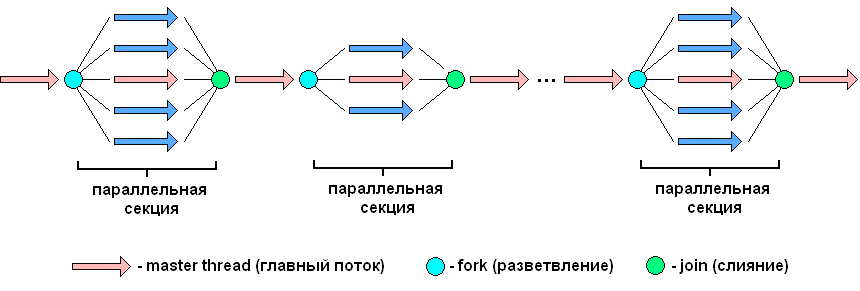
\includegraphics[width=0.9\textwidth]{../resources/openMP}
    \end{center}
    \caption{Схема работы OpenMP.}
\end{figure}
